%\clearpage
\section{Patentanalyse}\label{sec:Patentanalyse}
\subsection{Beschreibung}\label{subsec:Beschreibung}
Bei dem Patent Planta wird ein freischwingendes Schaltnetzteil beschrieben. Dieses Netzteil enthält folgende Baugruppen, ein Transformator mit einer Leistungswicklung zur Bereitstellung einer Ausgangsspannung, eine Treiberwicklung zur Bereitstellung einer Schaltspannung und eine Reglerwicklung zur Bereitstellung einer Messspannung. Die Ausgangsspannung kann mit Hilfe einer Abschaltspannung von einem Transistor geändert werden. Ein Gleichrichter empfängt die Messspannung und erzeugt eine für die Messspannung repräsentative Steuerspannung. Ein erster Spannungsteiler empfängt die Steuerspannung und schaltet den Schalttransistor ein, wenn die Sperrspannung über einem ersten Schwellwert liegt. Ein zweiter Spannungsteiler empfängt die Steuerspannung und schaltet den Schalttransistor aus, wenn die Sperrspannung unter einem zweiten Schwellwert liegt. Mit diesem Schaltnetzteil wird mit einer Primärsteuerung eine wirksame Spannungsstabilisierung mit einem guten Wirkungsgrad geboten.


\subsection{Schema}\label{subsec:Schema}
\begin{figure}[h!]
	\centering
	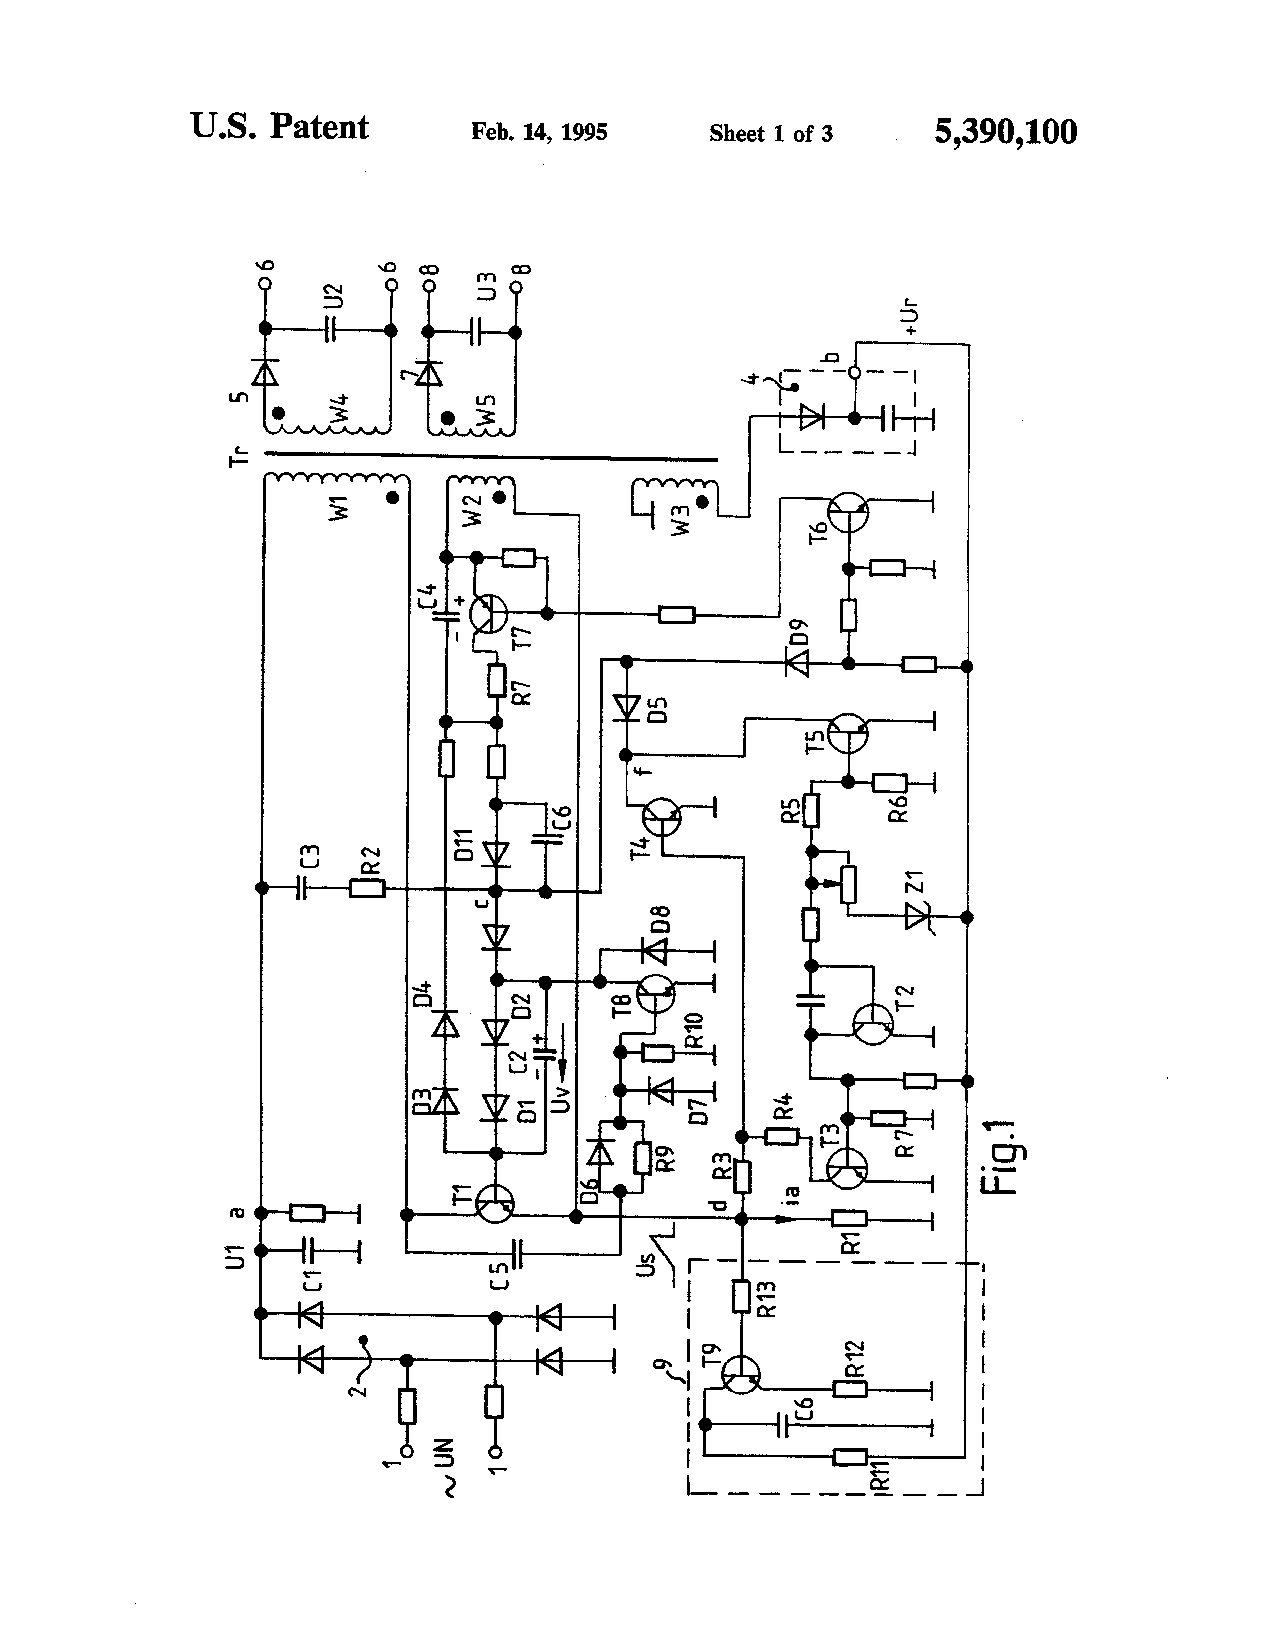
\includegraphics[width=1\textwidth]{graphics/Schema}
	\caption{Schema}
	\label{fig:Schema}
\end{figure} 
\newpage
\subsection{Claim-Chart}\label{sec:Claim-Chart}
\begin{tabular}{|l|l|l|}
	\hline 
\textbf{US5390100 Planta Claim 1}& &    \\ 
	\hline 
Ein frei schwingendes Schaltnetzteil, bestehend aus:	&  &  \\ 
	\hline 
einem Transformator mit einer Primärwicklung, einer Sekundärwicklung zur& A &  \\ Bereitstellung einer Ausgangsspannung und einer Regelwicklung zur&  &  \\
Bereitstellung einer Messspannung & &	 \\
	\hline 
einen Schalttransistor mit einer Abschaltspannung, der mit der & B & \\
Primärwicklung gekoppelt ist, um den Strom darin zu steuern	&  &  \\ 
	\hline 
Mittel zum Erzeugen einer mit der Messspannung gekoppelten Steuerspannung	& C &  \\ 
	\hline 
erste Rückkopplungsmittel zum Variieren der Abschaltspannung als Reaktion & D &\\
auf die Steuerspannung, wenn die Steuerspannung einen ersten Schwellenwert & &\\
überschreitet	&  &  \\ 
	\hline 
eine zweite Rückkopplungseinrichtung, die auf die Steuerspannung anspricht, & E &\\
um den Burst-Modus-Betrieb des Schalttransistors einzuleiten, wenn die & &\\
Steuerspannung einen zweiten Schwellenwert überschreitet.	&  &  \\ 
	\hline 

\end{tabular} 

\begin{figure}[h!]
	\centering
	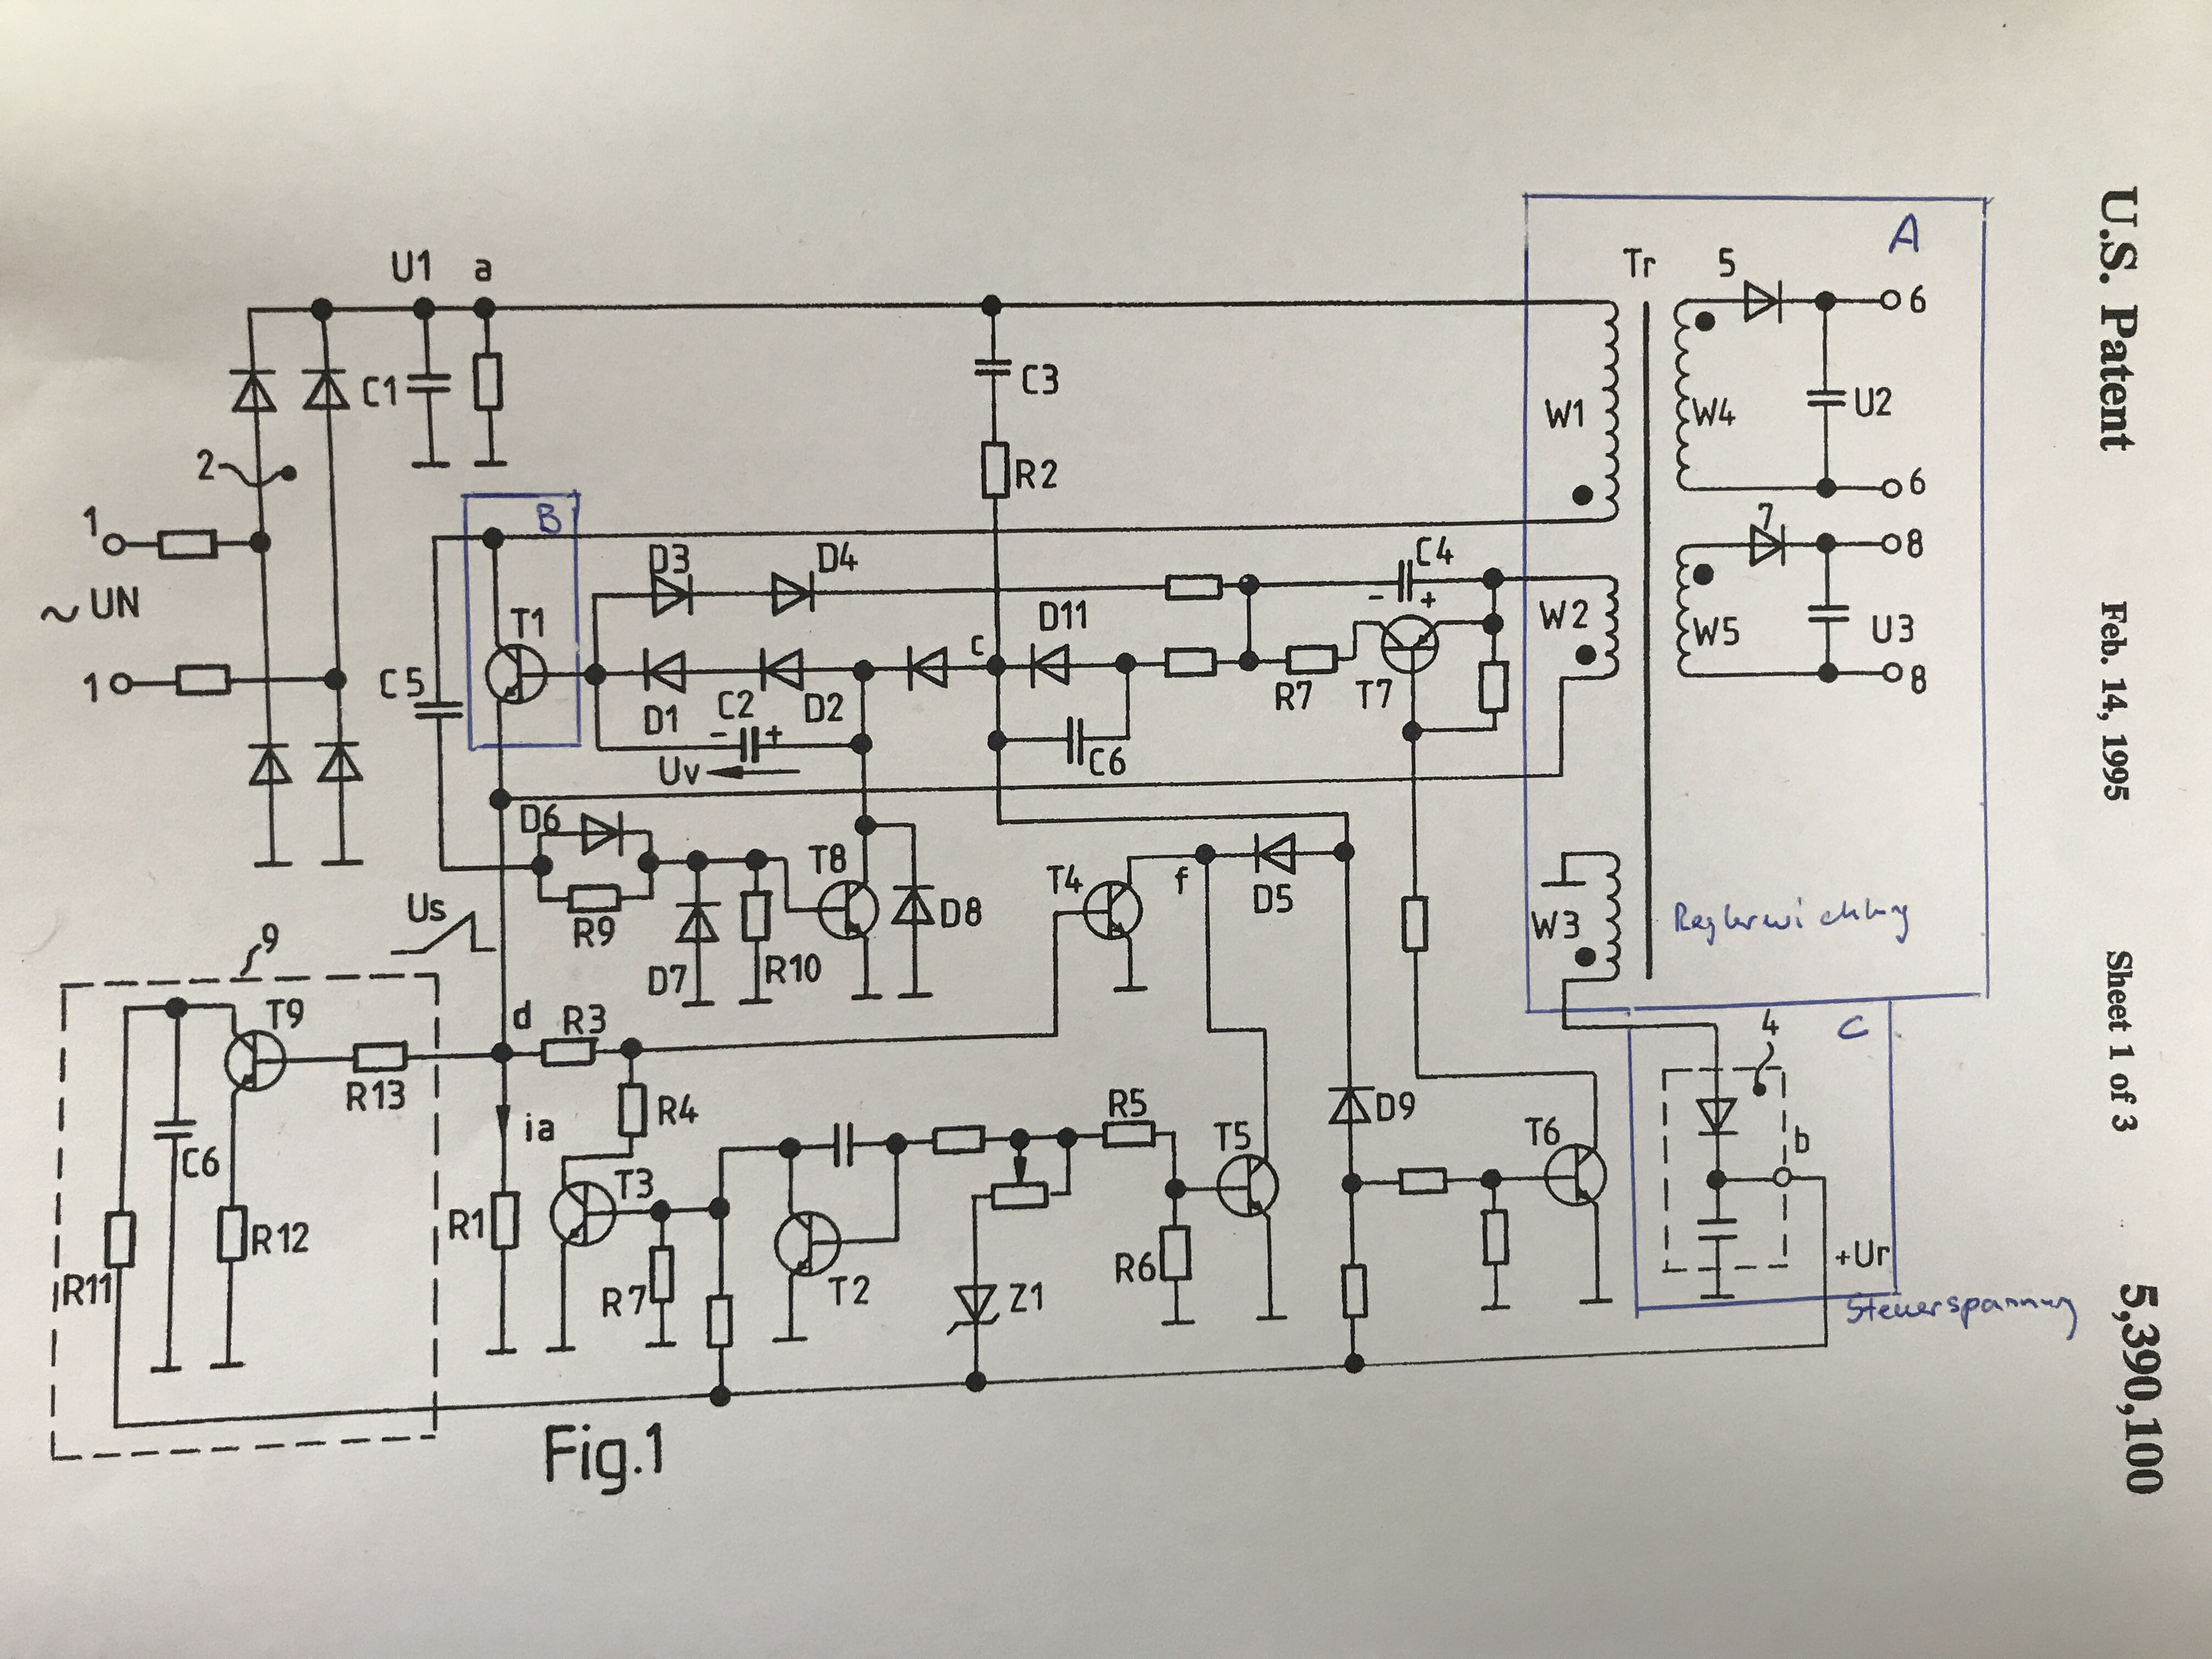
\includegraphics[width=1\textwidth]{graphics/CCHSchema}
	\caption{Claim Chart Schema}
	\label{fig:CCHSchema}
\end{figure} 